\documentclass[]{report}
\usepackage{amsmath}
\usepackage{amssymb}
\usepackage[english]{babel}
\usepackage[utf8]{inputenc}
\usepackage[T1]{fontenc}
\usepackage{euler}

\usepackage[inner=0cm,outer=0cm,top=0.1cm,bottom=0cm,paperwidth=9.3cm,paperheight=3.9cm]{geometry}

\usepackage{tikz,pgfplots}
\usetikzlibrary{positioning}
\usetikzlibrary{decorations.pathmorphing}

\begin{document}
\centering
	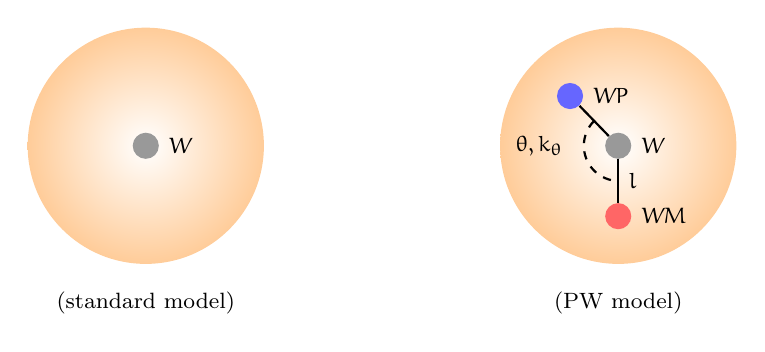
\begin{tikzpicture}
		%\draw[gray,step=1] (-6,-3) grid (6,3);
		\shade[inner color=white,outer color=orange!40] (-3,0) circle (1.5);
		\node[fill=gray!80, circle, radius=0.4, label=right:\footnotesize$W$] at (-3,0) {};
		\shade[inner color=white,outer color=orange!40] (3,0) circle (1.5);
		\node[fill=gray!80, circle, radius=0.4, label=right:\footnotesize$W$] (W) at (3,0) {};
		\node[fill=blue!60, circle, radius=0.4, label=right:\footnotesize$WP$] (WP) at (2.388, 0.632) {};
		\node[fill=red!60, circle, radius=0.4, label=right:\footnotesize$WM$] (WM) at (3,-0.894) {};
		\draw[thick] (W) -- (WP);
		\draw[thick] (W) -- (WM) node[midway,right]{\footnotesize $l$};
		\draw[dashed,thick] (2.694,0.316) arc [start angle=135, end angle=270, x radius=0.447, y radius=0.447];
		\node[] at (2,0) {\footnotesize$\theta,k_\theta$};
		\node[] at (-3,-2){\footnotesize (standard model)};
		\node[] at (3,-2){\footnotesize (PW model)};
	\end{tikzpicture}
\end{document}
	